% CSC3218 — Technical report (compile with pdflatex twice for TOC).
% Figures: ../results/   | Optional logo: place ucu_logo.png in this folder (same directory as this .tex)

\documentclass[11pt,a4paper]{article}
\usepackage[margin=2.2cm]{geometry}
\usepackage{graphicx}
\usepackage{booktabs}
\usepackage{hyperref}
\usepackage{amsmath}
\usepackage{appendix}
\usepackage{enumitem}
\usepackage{parskip}
\setlength{\parskip}{0.45em}
\setlength{\parindent}{0pt}
\hypersetup{colorlinks=true, linkcolor=blue!55!black, urlcolor=blue!55!black, citecolor=blue!55!black}

\begin{document}

% ---------- Cover page ----------
\begin{titlepage}
  \centering
  \vspace*{0.8cm}

  \IfFileExists{ucu_logo.png}{%
    \includegraphics[width=4.2cm]{ucu_logo.png}\\[1.2cm]%
  }{%
    {\Large\scshape Uganda Christian University}\\[0.6cm]%
    \rule{0.72\textwidth}{0.6pt}\\[0.45cm]%
  }

  {\large\bfseries Faculty of Engineering, Design and Technology}\\[1.8cm]

  {\LARGE\bfseries CIFAR-10 Image Classification\\[0.35em]
  using a Convolutional Neural Network}\\[0.8cm]

  {\large\itshape CSC3218 --- Deep Learning}\\[0.35cm]
  {\normalsize Technical / Laboratory Report}\\[2.2cm]

  \begin{tabular}{@{}rl@{}}
    \textbf{Name:} & Geno Owor Joshua \\[0.6em]
    \textbf{Registration No.:} & M23B23/006 \\
  \end{tabular}

  \vfill
  {\large \today}
\end{titlepage}

\newpage
\tableofcontents
\newpage

% ---------- Abstract ----------
\begin{abstract}
\noindent
This report documents an end-to-end deep learning experiment on the CIFAR-10 benchmark. We design a convolutional neural network (CNN) with batch normalization, dropout, and global average pooling, trained with AdamW, learning-rate reduction on validation accuracy, and early-stopping logic. Data augmentation is applied only to the training subset; a held-out validation split guides model selection without using the official test set during training. The best model achieves \textbf{91.67\%} accuracy on the CIFAR-10 test set, with discussion of overfitting indicators, per-class behaviour, and possible extensions (e.g.\ residual architectures).
\end{abstract}

\section{Introduction}

\subsection{Context}
Image classification is the task of assigning a discrete category label to an input image. Convolutional neural networks (CNNs) are the standard approach for natural-image classification because they encode \emph{local}, \emph{translation-aware} structure: early layers detect edges and textures, while deeper layers compose parts and object-level cues through stacking of convolutions, non-linearities, and pooling.

\subsection{Problem statement}
Given a colour image $\mathbf{x} \in \mathbb{R}^{3\times 32\times 32}$, we predict one of ten CIFAR-10 object classes. The model outputs logits $\mathbf{z}\in\mathbb{R}^{10}$; probabilities are $\mathrm{softmax}(\mathbf{z})_k = e^{z_k}/\sum_j e^{z_j}$. Training minimizes the cross-entropy between the true one-hot label and the predicted distribution; in PyTorch, \texttt{CrossEntropyLoss} combines \texttt{log\_softmax} and negative log-likelihood for numerical stability.

\subsection{Objectives}
The objectives of this work are to:
\begin{itemize}[noitemsep]
  \item implement a reproducible CIFAR-10 pipeline (load, split, augment, normalize);
  \item build a custom CNN meeting coursework design constraints (convolution, batch norm, pooling, dropout, global pooling, classifier);
  \item train with modern optimization and regularization (AdamW, weight decay, augmentation, optional early stopping);
  \item report quantitative metrics (accuracy, macro precision/recall/F1) and qualitative analysis (curves, confusion matrix, sample predictions).
\end{itemize}

\subsection{Report structure}
Section~\ref{sec:dataset} describes the dataset and preprocessing. Section~\ref{sec:method} details the architecture and training protocol. Section~\ref{sec:exp} summarises the experimental setup. Section~\ref{sec:results} presents results; Section~\ref{sec:disc} discusses limitations and improvements. Section~\ref{sec:conc} concludes. An appendix lists per-class test metrics.

\section{Dataset and preprocessing}
\label{sec:dataset}

\subsection{CIFAR-10}
The Canadian Institute For Advanced Research (CIFAR)-10 dataset contains 60{,}000 $32\times 32$ RGB images, 6{,}000 per class, with labels in ten mutually exclusive categories: airplane, automobile, bird, cat, deer, dog, frog, horse, ship, and truck. The \emph{official} partition is 50{,}000 training images and 10{,}000 test images. All classes are balanced.

\subsection{Train / validation / test protocol}
We \textbf{do not} tune hyperparameters on the official test set. From the 50{,}000 training images we reserve \textbf{10\%} as a \textbf{validation} set (5{,}000 images) using a fixed random seed (42) for reproducibility. The remaining \textbf{90\%} (45{,}000 images) are used for parameter updates. The official \textbf{10{,}000} test images are used \textbf{once} for final reporting after training.

\subsection{Normalization}
Each image is converted to a tensor in $[0,1]$ per channel, then standardized with dataset-wide means $(0.4914, 0.4822, 0.4465)$ and standard deviations $(0.2470, 0.2435, 0.2616)$ per RGB channel. These statistics are standard for CIFAR-10 and stabilize optimization.

\subsection{Data augmentation (training only)}
On the training subset only, we apply:
\begin{itemize}[noitemsep]
  \item \textbf{RandomCrop}($32$, padding=$4$): simulates small translation and scale;
  \item \textbf{RandomHorizontalFlip}(): exploits left--right symmetry for many object categories.
\end{itemize}
Validation and test pipelines use \textbf{only} normalization (no random transforms), avoiding leakage of augmented statistics into evaluation.

\section{Methodology}
\label{sec:method}

\subsection{CNN architecture}
\label{sec:arch}
We use a custom \texttt{CIFAR10CNN} with three spatial stages. Each stage contains \textbf{two} $3\times 3$ convolutional layers (same padding), each followed by \textbf{batch normalization} and \textbf{ReLU}. After the second conv block in each stage, we apply $2\times 2$ \textbf{max pooling} (halving spatial size) and \textbf{dropout} on feature maps (scaled dropout rate in early stages). Channel depths are \textbf{64 $\to$ 128 $\to$ 256}. After the third stage, spatial resolution is $4\times 4$; \textbf{global average pooling} (GAP) reduces each channel to a scalar, yielding a 256-dimensional vector. The \textbf{classifier} is: linear(256$\to$128) $\to$ batch norm $\to$ ReLU $\to$ dropout $\to$ linear(128$\to$10 logits).

GAP reduces parameter count compared to flattening large feature maps and encourages learning of class-salient channel activations. Dropout and weight decay address overfitting on the relatively small CIFAR images.

\subsection{Loss and optimization}
The training loss is \textbf{cross-entropy} for multi-class classification. Optimization uses \textbf{AdamW} (decoupled weight decay) with learning rate $\alpha = 3\times 10^{-4}$ and weight decay $\lambda = 10^{-4}$. We use \textbf{ReduceLROnPlateau}, monitoring \textbf{validation accuracy}, with factor $0.5$ and patience \textbf{4} epochs: if validation accuracy stagnates, the learning rate is multiplied by $0.5$.

\subsection{Early stopping}
We track the best validation accuracy and save the corresponding weights. If validation accuracy does not \textbf{strictly improve} for \textbf{12} consecutive epochs, training would stop early and reload the best checkpoint. In the reported run, training completed the full \textbf{80} epoch budget (early stopping did not terminate earlier).

\section{Experimental setup}
\label{sec:exp}

Table~\ref{tab:hyper} summarises hyperparameters and environment. Training was executed on \textbf{CPU}; wall-clock time was approximately \textbf{18.6~hours} ($\sim 6.67\times 10^4$~s). A GPU would reduce epoch time but does not change the methodological narrative.

\begin{table}[ht]
  \centering
  \caption{Hyperparameters and run configuration.}
  \label{tab:hyper}
  \begin{tabular}{@{}ll@{}}
    \toprule
    Setting & Value \\
    \midrule
    Batch size & 64 \\
    Max epochs & 80 (all completed) \\
    Optimizer & AdamW ($\alpha=3\times 10^{-4}$, $\lambda=10^{-4}$) \\
    LR scheduler & ReduceLROnPlateau (factor 0.5, patience 4) \\
    Early-stop patience & 12 epochs (no improvement on val acc) \\
    Dropout (classifier / spatial) & 0.3 (scaled in early blocks) \\
    Train / val split & 90\% / 10\% of 50k \\
    Random seed & 42 \\
    DataLoader workers & 2 \\
    Framework & PyTorch \\
    Device & CPU \\
    \bottomrule
  \end{tabular}
\end{table}

\section{Results}
\label{sec:results}

\subsection{Overall test metrics}
On the \textbf{official test set} (10{,}000 images), the selected model achieves:
\begin{itemize}[noitemsep]
  \item \textbf{Accuracy:} 91.67\%;
  \item \textbf{Macro precision:} 91.63\%; \textbf{macro recall:} 91.67\%; \textbf{macro F1:} 91.62\%;
  \item \textbf{Test loss} (cross-entropy): $\approx 0.263$.
\end{itemize}

\subsection{Generalization gap}
On the \textbf{best validation checkpoint}, training accuracy reached \textbf{98.18\%} while validation accuracy was \textbf{92.16\%}. The gap between training and validation performance indicates \textbf{mild overfitting}, though validation and test accuracies are close (92.16\% vs.\ 91.67\%), suggesting the validation split was reasonably representative.

\subsection{Per-class test performance}
Table~\ref{tab:perclass} summarises precision, recall, and F1 per class (10{,}000 test samples, 1{,}000 per class). The lowest recall appears for \textit{cat} (78.7\%), consistent with fine-grained confusion with visually similar classes (e.g.\ \textit{dog}). Strong scores appear for \textit{automobile}, \textit{frog}, \textit{ship}, and \textit{truck}.

\begin{table}[ht]
  \centering
  \caption{Per-class precision, recall, and F1 on the CIFAR-10 test set.}
  \label{tab:perclass}
  \small
  \begin{tabular}{@{}lccc@{}}
    \toprule
    Class & Precision & Recall & F1 \\
    \midrule
    airplane   & 0.919 & 0.932 & 0.926 \\
    automobile & 0.968 & 0.958 & 0.963 \\
    bird       & 0.901 & 0.878 & 0.890 \\
    cat        & 0.866 & 0.787 & 0.825 \\
    deer       & 0.900 & 0.929 & 0.914 \\
    dog        & 0.859 & 0.877 & 0.868 \\
    frog       & 0.940 & 0.942 & 0.941 \\
    horse      & 0.936 & 0.947 & 0.941 \\
    ship       & 0.938 & 0.959 & 0.949 \\
    truck      & 0.936 & 0.958 & 0.947 \\
    \midrule
    \textbf{Macro avg} & \textbf{0.916} & \textbf{0.917} & \textbf{0.916} \\
    \bottomrule
  \end{tabular}
\end{table}

\begin{figure}[ht]
  \centering
  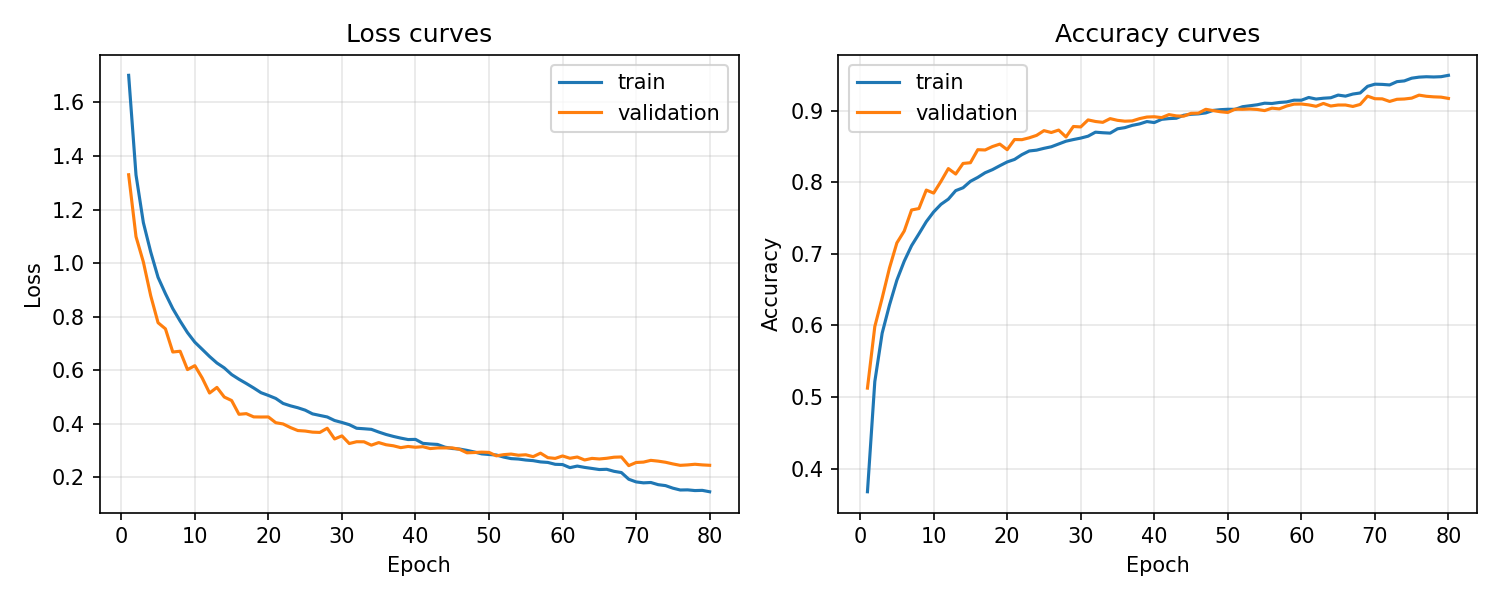
\includegraphics[width=\linewidth]{../results/curves_loss_accuracy.png}
  \caption{Training vs.\ validation loss and accuracy per epoch (80 epochs).}
  \label{fig:curves}
\end{figure}

\begin{figure}[ht]
  \centering
  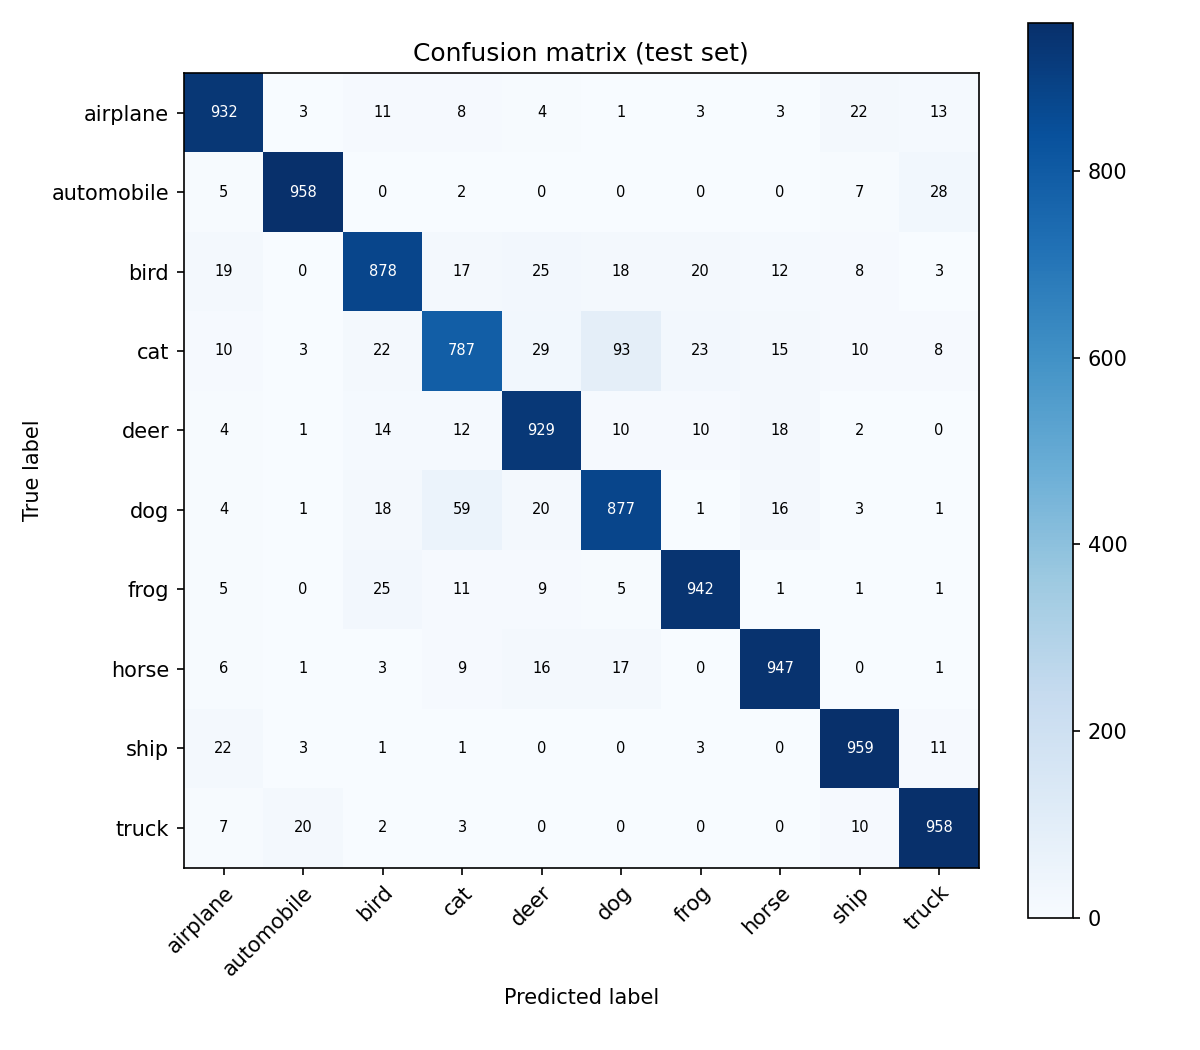
\includegraphics[width=0.88\linewidth]{../results/confusion_matrix_test.png}
  \caption{Confusion matrix on the official test set (counts per true vs.\ predicted class).}
  \label{fig:cm}
\end{figure}

\begin{figure}[ht]
  \centering
  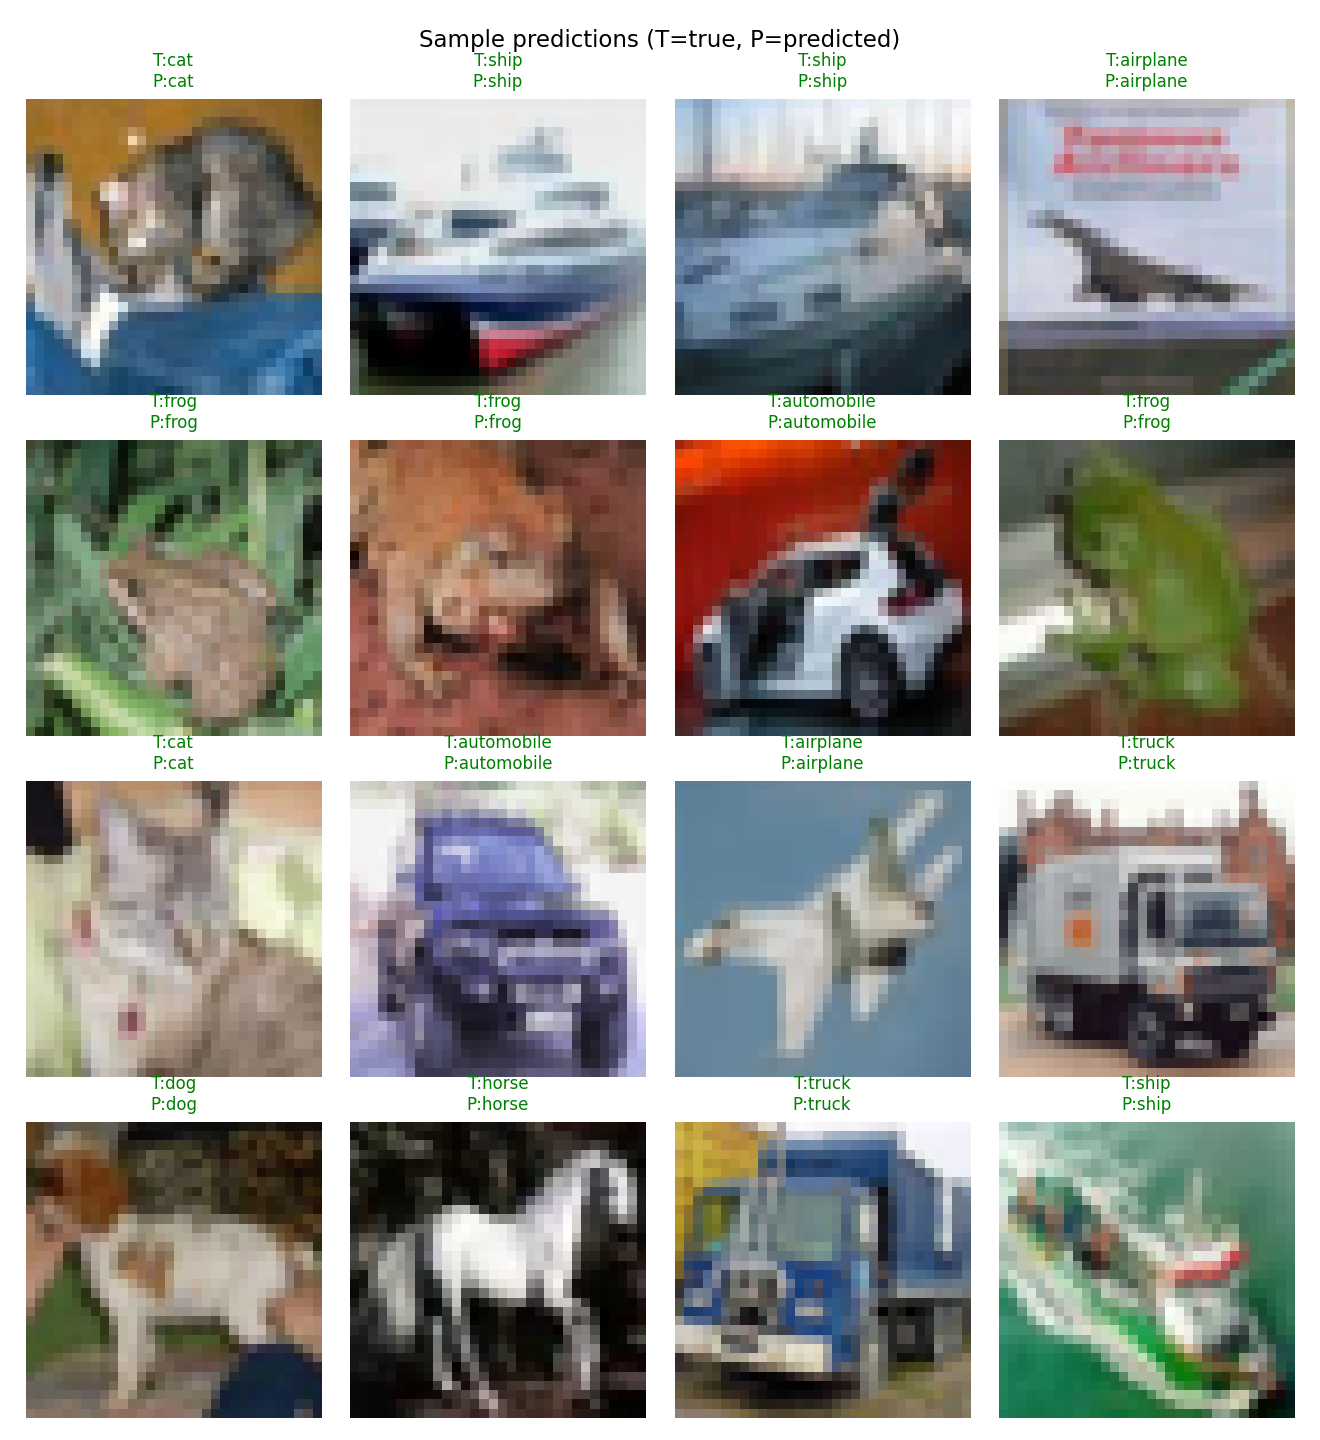
\includegraphics[width=\linewidth]{../results/sample_predictions.png}
  \caption{Sample test predictions: \textbf{green} titles indicate correct predictions; \textbf{red} indicate errors.}
  \label{fig:samples}
\end{figure}

\section{Discussion}
\label{sec:disc}

Figure~\ref{fig:curves} shows that training loss decreases steadily and training accuracy approaches saturation, while validation metrics improve more slowly and plateau, which is typical for CNNs on CIFAR-10 with moderate capacity. The train--validation gap supports the use of \textbf{regularization} (dropout, weight decay, augmentation) and monitoring validation rather than training accuracy for model selection.

The confusion matrix (Figure~\ref{fig:cm}) and Table~\ref{tab:perclass} highlight \textbf{inter-class confusion}, especially around mammals and small objects. Sample predictions (Figure~\ref{fig:samples}) illustrate both confident correct predictions and plausible mistakes (e.g.\ texture or pose ambiguity).

\textbf{Possible improvements} include: residual networks (ResNet) or wider architectures; stronger augmentation (cutout, RandAugment, mixup); cosine or one-cycle learning-rate schedules; label smoothing; longer training with careful tuning; test-time augmentation; and transfer learning from larger datasets (not required for the baseline assignment but common in practice).

\section{Conclusion}
\label{sec:conc}
We implemented and trained a batch-normalized, dropout-regularized CNN with global average pooling on CIFAR-10, using a proper train/validation/test protocol. The model reached \textbf{91.67\%} test accuracy with balanced macro-averaged precision and recall. Learning curves, a confusion matrix, and qualitative samples together explain \emph{how well} the model performs and \emph{where} it fails. Future work could target harder classes and reduce the train--validation gap through architecture and augmentation upgrades.

\begin{thebibliography}{9}
\bibitem{krizhevsky2009}
A.~Krizhevsky, ``Learning multiple layers of features from tiny images,'' University of Toronto, technical report, 2009. (CIFAR-10 dataset.)
\bibitem{pytorch}
A.~Paszke \emph{et al.}, ``PyTorch: An imperative style, high-performance deep learning library,'' NeurIPS, 2019.
\bibitem{loshchilov2019}
I.~Loshchilov and F.~Hutter, ``Decoupled weight decay regularization,'' ICLR, 2019. (AdamW.)
\end{thebibliography}

\begin{appendices}
\section{Replication notes}
\label{app:rep}
Code and outputs are produced with the project scripts: \texttt{train.py} writes \texttt{results/metrics.json}, \texttt{classification\_report.txt}, and figure files referenced above. Compiling this document from the \texttt{report/} directory expects figures at \texttt{../results/}. To show the UCU emblem on the cover, save the official logo as \texttt{report/ucu\_logo.png} (same folder as this \texttt{.tex} file); if the file is absent, a text header is shown instead.

\section{Sklearn classification report excerpt (test set)}
\label{app:sk}
\small
\begin{verbatim}
              precision    recall  f1-score   support
    airplane     0.9191    0.9320    0.9255      1000
  automobile     0.9677    0.9580    0.9628      1000
        bird     0.9014    0.8780    0.8896      1000
         cat     0.8658    0.7870    0.8245      1000
        deer     0.9002    0.9290    0.9144      1000
         dog     0.8590    0.8770    0.8679      1000
        frog     0.9401    0.9420    0.9411      1000
       horse     0.9358    0.9470    0.9414      1000
        ship     0.9384    0.9590    0.9486      1000
       truck     0.9355    0.9580    0.9466      1000
    accuracy                         0.9167     10000
   macro avg     0.9163    0.9167    0.9162     10000
weighted avg     0.9163    0.9167    0.9162     10000
\end{verbatim}
\end{appendices}

\end{document}
